\documentclass[11pt,a4paper]{article}

% ---------- Encodage / langue ----------
\usepackage[utf8]{inputenc}
\usepackage[T1]{fontenc}
\usepackage[french,provide=*]{babel}
\usepackage[margin=2.2cm]{geometry}

% ---------- Feuille de style fournie ----------
\usepackage{ancien_style_de_cours_gaspard}
\usepgfplotslibrary{fillbetween}

% ---------- Compteur local pour numéroter les exemples ----------
\newcounter{exemplenum}
\newcommand{\exnum}{\stepcounter{exemplenum}\textbf{Exemple~\theexemplenum.} }

\setlength{\parindent}{0pt}
\setlength{\parskip}{4pt}

\begin{document}

% ================= TITRE =================
\begin{center}
{\large\textsc{BTS SBM -- 2\textsuperscript{e} année}}\\[2pt]
{\Huge\bfseries\blueuline{Lois de probabilité}}
\end{center}
\bigskip

% ========================================================
\section{Variables aléatoires discrètes}

\subsection{Loi de probabilité}

\begin{definition}
Une \textbf{variable aléatoire} $X$ associe un nombre à chaque issue d'une expérience aléatoire. Lorsque $X$ ne prend qu'un nombre fini de valeurs $x_1,\dots,x_n$, la \textbf{loi de probabilité} de $X$ donne, pour chaque valeur $x_i$, la probabilité $p_i = P(X=x_i)$ (avec toujours $p_1+\cdots+p_n=1$). On peut la représenter par un tableau ou par un \textbf{diagramme en bâtons}.
\end{definition}

\subsection{Espérance et écart-type}

\begin{definition}
L'\textbf{espérance} $E(X)$ est la valeur moyenne théorique de $X$~; l'\textbf{écart-type} $\sigma(X)$ mesure la dispersion des valeurs autour de cette moyenne. On les obtient directement à la \textbf{calculatrice} (mode statistique~: valeurs $x_i$ en liste 1, probabilités $p_i$ en liste 2).
\end{definition}

\subsection{Un exemple important~: la loi binomiale}

\begin{definition}
Une expérience aléatoire à deux issues, l'une appelée \textbf{succès} (de probabilité $p$) et l'autre \textbf{échec}, est une \textbf{épreuve de Bernoulli}. Lorsqu'on répète $n$ fois, de façon indépendante, la même épreuve de Bernoulli, et que $X$ compte le nombre de succès obtenus, on dit que $X$ suit une \textbf{loi binomiale} de paramètres $n$ et $p$, notée $X \sim \mathcal{B}(n,p)$.
\end{definition}

\begin{methode}{Calculer une probabilité binomiale à la calculatrice}
Les calculatrices possèdent une fonction dédiée à la loi binomiale (menu \textit{Loi} ou \textit{Distr}, puis \textit{Binomiale})~: il suffit d'indiquer $n$, $p$ et la valeur de $k$ recherchée pour obtenir directement $P(X=k)$, sans avoir à poser de calcul.
\end{methode}

\begin{propriete}
Si $X \sim \mathcal{B}(n,p)$, alors~:
$$E(X) = np \qquad \text{et} \qquad \sigma(X) = \sqrt{np(1-p)}$$
\end{propriete}

\begin{exemple}
\exnum On lance $20$ fois un dé équilibré à six faces et on note $X$ le nombre de fois où l'on obtient un $6$. Les lancers étant indépendants, $X$ suit la loi binomiale $\mathcal{B}\left(20~;~\dfrac{1}{6}\right)$.

À la calculatrice, on trouve $P(X=3) \approx 0{,}238$. Avec la propriété ci-dessus~:
$$E(X) = 20 \times \dfrac{1}{6} \approx 3{,}33 \qquad \sigma(X) = \sqrt{20 \times \dfrac{1}{6}\times\dfrac{5}{6}} \approx 1{,}67$$

Voici le diagramme en bâtons de cette loi~:

\begin{center}
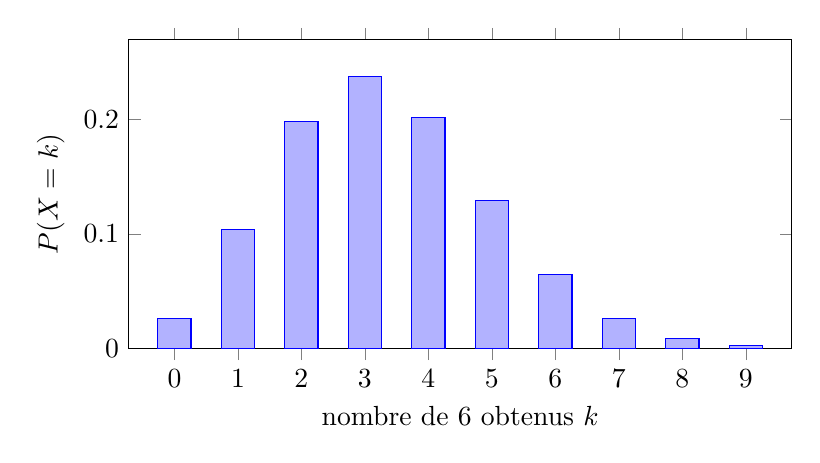
\begin{tikzpicture}
\begin{axis}[
  width=10cm, height=5.5cm,
  ybar, bar width=12pt,
  ymin=0, ymax=0.27,
  xtick=data,
  xlabel={nombre de $6$ obtenus $k$}, ylabel={$P(X=k)$},
  enlarge x limits=0.08,
]
\addplot[fill=blue!30,draw=blue] coordinates {
(0,0.0261) (1,0.1043) (2,0.1982) (3,0.2379) (4,0.2022)
(5,0.1294) (6,0.0647) (7,0.0259) (8,0.0084) (9,0.0022)};
\end{axis}
\end{tikzpicture}
\end{center}

On observe que ce diagramme, avec $p=\frac16$ petit, est dissymétrique.
\end{exemple}

\begin{exo}
\textit{Utiliser la loi binomiale à la calculatrice}
\medskip

\textbf{Énoncé.} Dans une usine, $5\,\%$ des pièces produites sont défectueuses. On prélève au hasard un échantillon de 15 pièces dans une très grande production (on peut assimiler ce prélèvement à des tirages indépendants). Soit $X$ le nombre de pièces défectueuses parmi les 15 prélevées.
\begin{enumerate}[leftmargin=6mm]
\item Justifier que $X$ suit une loi binomiale et donner ses paramètres.
\item À la calculatrice, calculer $P(X=2)$.
\item Calculer $E(X)$ et $\sigma(X)$.
\item Calculer $P(X \leqslant 1)$ et interpréter le résultat.
\end{enumerate}

\textbf{Solution.}

\textbf{1.} On répète $n=15$ fois, de façon indépendante, la même épreuve de Bernoulli (« la pièce est défectueuse », de probabilité $p=0{,}05$)~: $X \sim \mathcal{B}(15~;~0{,}05)$.

\textbf{2.} À la calculatrice, $P(X=2) \approx 0{,}135$.

\textbf{3.} $E(X) = 15 \times 0{,}05 = 0{,}75$ et $\sigma(X) = \sqrt{15\times0{,}05\times0{,}95} \approx 0{,}84$.

\textbf{4.} À la calculatrice, $P(X \leqslant 1) \approx 0{,}829$. Il y a donc environ $83\,\%$ de chances qu'il y ait au plus une pièce défectueuse dans l'échantillon.
\end{exo}

% ========================================================
\section{loi normale}

\subsection{Loi normale, une approximation de la loi binomiale}

\begin{remarque}
Reprenons la loi binomiale, mais avec $p=0{,}5$~: voici le diagramme en bâtons de $\mathcal{B}(20~;~0{,}5)$~:

\begin{center}
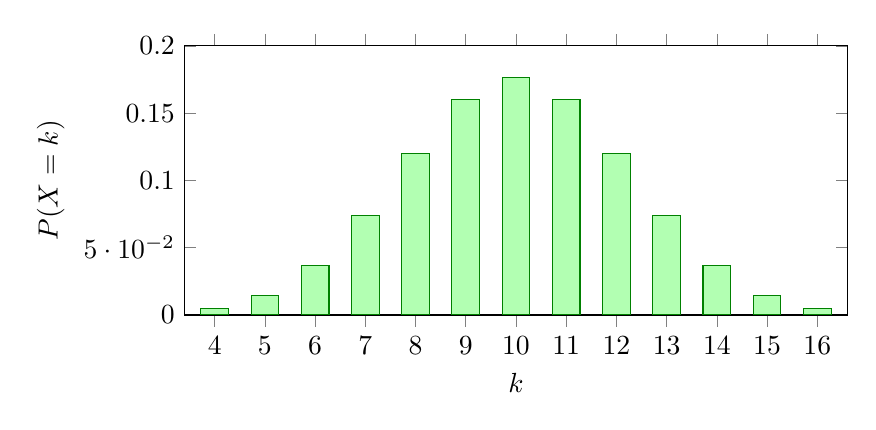
\begin{tikzpicture}
\begin{axis}[
  width=10cm, height=5cm,
  ybar, bar width=10pt,
  ymin=0, ymax=0.2,
  xtick=data,
  xlabel={$k$}, ylabel={$P(X=k)$},
  enlarge x limits=0.05,
]
\addplot[fill=green!30,draw=green!50!black] coordinates {
(4,0.0046) (5,0.0148) (6,0.037) (7,0.0739) (8,0.1201) (9,0.1602)
(10,0.1762) (11,0.1602) (12,0.1201) (13,0.0739) (14,0.037) (15,0.0148) (16,0.0046)};
\end{axis}
\end{tikzpicture}
\end{center}

Ce diagramme a une allure « en cloche », symétrique~: pour $n$ grand, on peut approcher la loi binomiale par une loi \textbf{continue}, la \textbf{loi normale}.
\end{remarque}

\begin{propriete}
\textit{(admise)} Si $X \sim \mathcal{B}(n,p)$ avec $n$ suffisamment grand (en pratique, on demande $np \geqslant 5$ et $n(1-p)\geqslant5$), alors on peut approcher la loi de $X$ par la loi normale de \textbf{même espérance et même écart-type} que $X$, c'est-à-dire $\mathcal{N}\big(np~;~\sqrt{np(1-p)}\,\big)$.
\end{propriete}

\begin{definition}
Plus généralement, une variable aléatoire $X$ suit une \textbf{loi normale} d'espérance $m$ et d'écart-type $\sigma$, notée $X \sim \mathcal{N}(m\,;\,\sigma)$, lorsque sa courbe est la célèbre « \textbf{courbe en cloche} »~: une courbe symétrique, centrée en $m$, dont la largeur dépend de $\sigma$ (plus $\sigma$ est grand, plus la cloche est étalée).
\end{definition}

\begin{center}
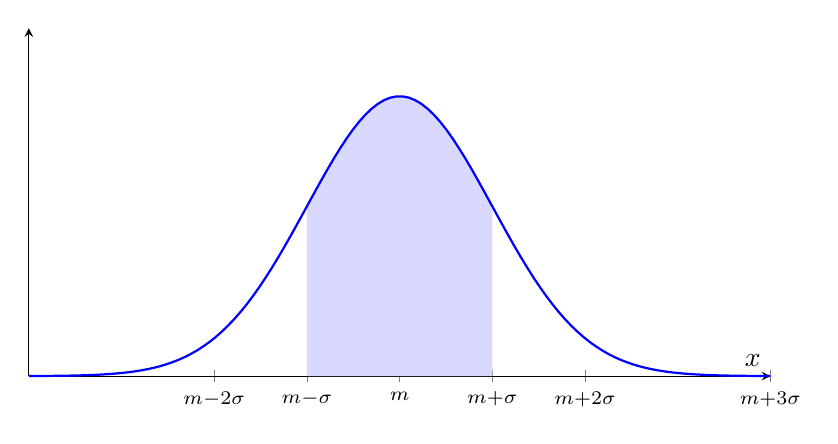
\begin{tikzpicture}
\begin{axis}[
  width=11cm, height=6cm,
  axis lines=middle,
  xlabel={$x$}, ylabel={},
  xtick={26.8,28.4,29.2,30,30.8,31.6,33.2},
  xticklabels={$m{-}3\sigma$,$m{-}2\sigma$,$m{-}\sigma$,$m$,$m{+}\sigma$,$m{+}2\sigma$,$m{+}3\sigma$},
  x tick label style={font=\scriptsize},
  ytick=\empty,
  ymin=0, ymax=0.62,
  domain=26.8:33.2, samples=120,
  enlargelimits=false,
  clip=false
]
\addplot[name path=courbe, thick, blue, domain=26.8:33.2] {1/(0.8*sqrt(2*pi))*exp(-((x-30)^2)/(2*0.8^2))};
\path[name path=axe] (axis cs:29.2,0) -- (axis cs:30.8,0);
\addplot[blue!15] fill between[of=courbe and axe, soft clip={domain=29.2:30.8}];
\end{axis}
\end{tikzpicture}
\end{center}

\begin{propriete}
\textit{Règle empirique.} Si $X \sim \mathcal{N}(m\,;\,\sigma)$, alors, quelle que soit la loi normale considérée~:
$$P(m-\sigma \leqslant X \leqslant m+\sigma) \approx 0{,}68 \qquad P(m-2\sigma \leqslant X \leqslant m+2\sigma) \approx 0{,}95 \qquad P(m-3\sigma \leqslant X \leqslant m+3\sigma) \approx 0{,}997$$
(zone bleutée ci-dessus~: probabilité $\approx 0{,}68$ entre $m-\sigma$ et $m+\sigma$).
\end{propriete}


\begin{exo}
\textit{Utiliser la loi normale}
\medskip

\textbf{Énoncé.} La masse $X$ (en g) des baguettes produites par une boulangerie industrielle suit la loi normale $\mathcal{N}(250\,;\,3)$.
\begin{enumerate}[leftmargin=6mm]
\item Donner un intervalle centré en $250$ contenant environ $95\,\%$ des baguettes produites.
\item Une baguette est déclarée non conforme si sa masse n'appartient pas à $[244\,;\,256]$. Cet intervalle correspond-il à environ $95\,\%$ ou $99{,}7\,\%$ de la production~? Justifier.
\item À l'aide de la calculatrice, donner $P(248 \leqslant X \leqslant 253)$.
\end{enumerate}

\textbf{Solution.}

\textbf{1.} On utilise $P(m-2\sigma \leqslant X \leqslant m+2\sigma) \approx 0{,}95$ avec $m=250$ et $\sigma=3$~:
$$m-2\sigma = 250-6 = 244 \qquad m+2\sigma = 250+6 = 256$$
Donc environ $95\,\%$ des baguettes ont une masse dans $[244\,;\,256]$.

\textbf{2.} On a $244 = 250-2\times3 = m-2\sigma$ et $256 = 250+2\times3 = m+2\sigma$~: il s'agit donc bien de l'intervalle correspondant à environ $95\,\%$ de la production (et non $99{,}7\,\%$, qui correspondrait à $[241\,;\,259]$).

\textbf{3.} À la calculatrice, on trouve $P(248 \leqslant X \leqslant 253) \approx 0{,}589$.
\end{exo}

\end{document}
